\section{The LACK Ontology}
\label{sec:ontology}

\paragraph{Ontology Engineering Methodology.}
The LACK ontology was designed following a bottom-up, requirements-driven process.
The starting point was an analysis of the knowledge needs raised by the investigative sources --- what types of relationships are expressed in DeSmog and LobbyMap profiles? --- which were formalised as a set of competency questions (CQ1--CQ12, see Section~\ref{sec:resource} and the LACK website\footnote{\url{https://climatesense-project.eu/lack/ontology.html}}).
These competency questions drove the design of the knowledge extraction pipeline described in Section~\ref{sec:extraction}, and were subsequently refined based on data quality assessment carried out at the end of the extraction process.
A guiding design principle throughout was to represent only what could be reliably and automatically produced by the extraction pipeline, deliberately excluding relation types that could not be extracted with sufficient confidence.
This constraint was essential to maximise the quality of a resource that cannot be fully verified manually and is intended to scale to very large volumes of data.

\paragraph{Motivation for a New Vocabulary.}
Two main considerations motivated the development of a new vocabulary rather than reusing an existing one.
First, existing general-purpose vocabularies such as schema.org do not adequately cover the domain-specific relationships present in climate lobbying data: the schema.org alignment exercise revealed systematic inverse direction mismatches and an absence of equivalents for lobbying-specific relations such as \emph{lobbied for}, \emph{conducted public relations for}, or \emph{incorporated}~\cite{schemaorg}.
Second, a key analytical goal of LACK is to support graph-based network analysis --- centrality, community detection, shortest path --- which requires direct typed links between entity nodes.
Schema.org's recommended pattern for named organisational roles (wrapping relations in materialised \texttt{schema:Role} intermediary nodes) would fragment the graph and complicate traversal, making it unsuitable for this purpose.

\paragraph{Top-Level Types.}
The ontology defines two top-level classes: \texttt{lack:Person}, representing an individual human being, and \texttt{lack:Collective}, representing any group of people organised around a shared purpose.
The choice of \texttt{Collective} over the more intuitive \texttt{Organisation} was motivated by quality analysis during extraction: the data revealed that many entities appearing in the sources were not organisations in the strict sense, but events (conferences, summits), journals, campaigns, committees, and networks.
Introducing \texttt{Collective} as a deliberately broad type accommodates this diversity without requiring the extraction pipeline to distinguish between multiple disjoint subclasses --- a distinction it could not make reliably.

\paragraph{Relation Types.}
Table~\ref{tab:ontology} provides a summary of the relation types defined in the ontology, grouped by category, and Figure~\ref{fig:ontology} shows the corresponding schema diagram.
Each relation is defined with a domain, a range, an inverse property, and where applicable a sub-property link within the hierarchy rooted at \texttt{lack:associatedWith} --- the top-level symmetric catch-all relation used when no more specific type applies.
The full vocabulary, including formal definitions and SPARQL examples for each competency question, is available on the LACK website\footnote{\url{https://climatesense-project.eu/lack/ontology.html}}.

\begin{figure}[th]
    \centering
    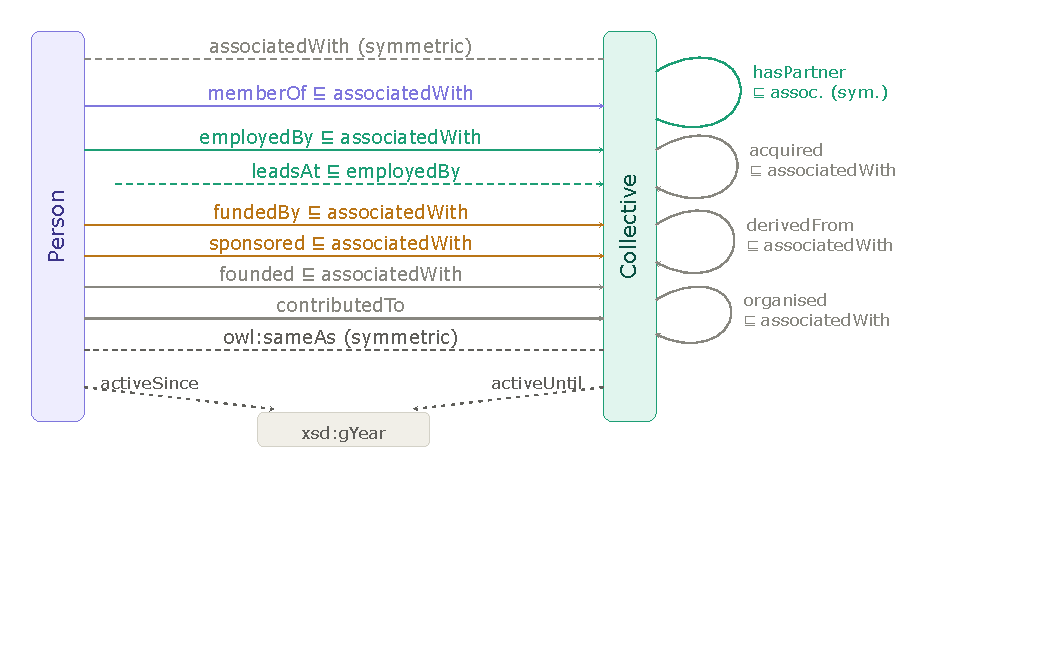
\includegraphics[width=\textwidth]{figures/lack-ontology-diagram.pdf}
    \caption{Schema diagram of the LACK ontology.}
    \label{fig:ontology}
\end{figure}

\begin{table}[t]
\caption{Summary of LACK relation types.}
\label{tab:ontology}
\centering
\small
\begin{tabular}{llllll}
\hline
\textbf{Group} & \textbf{Term} & \textbf{Domain} & \textbf{Range} & \textbf{Inverse} & \textbf{Sub-property of} \\
\hline
Membership   & \texttt{memberOf}      & Person      & Collective  & \texttt{hasMember}       & \texttt{associatedWith} \\
Employment   & \texttt{employedBy}    & Person      & Collective  & \texttt{hasEmployee}     & \texttt{associatedWith} \\
Leadership   & \texttt{leadsAt}       & Person      & Collective  & \texttt{hasLeader}       & \texttt{employedBy} \\
Funding      & \texttt{fundedBy}      & P $|$ C     & P $|$ C     & \texttt{hasFunder}       & \texttt{associatedWith} \\
Sponsorship  & \texttt{sponsored}     & P $|$ C     & P $|$ C     & \texttt{wasSponsoredBy}  & \texttt{associatedWith} \\
Founding     & \texttt{founded}       & P $|$ C     & Collective  & \texttt{wasFoundedBy}    & \texttt{associatedWith} \\
Contribution & \texttt{contributedTo} & P $|$ C     & Collective  & \texttt{hasContributor}  & --- \\
Partnership  & \texttt{hasPartner}    & Collective  & Collective  & (symmetric)              & \texttt{associatedWith} \\
Acquisition  & \texttt{acquired}      & Collective  & Collective  & \texttt{wasAcquiredBy}   & \texttt{associatedWith} \\
Derivation   & \texttt{derivedFrom}   & Collective  & Collective  & \texttt{hasDerivation}   & \texttt{associatedWith} \\
Association  & \texttt{associatedWith}& P $|$ C     & P $|$ C     & (symmetric)              & --- \\
Identity     & \texttt{owl:sameAs}    & P $|$ C     & P $|$ C     & (symmetric)              & --- \\
\hline
\end{tabular}
\end{table}

\noindent All \texttt{lack:} prefixes are omitted from the Term column for brevity. P = \texttt{lack:Person}, C = \texttt{lack:Collective}.

\paragraph{Reuse of External Vocabularies.}
Where established terms are available, the ontology reuses them rather than introducing new ones.
\texttt{owl:sameAs} is used to assert identity between entities --- covering renaming, aliases, and doing-business-as relations.
Provenance is represented using PROV-O~\cite{provo}: each reified statement is linked to a shared \texttt{prov:Activity} (the LACK extraction activity) and a \texttt{prov:SoftwareAgent} (the extraction pipeline), via \texttt{prov:wasGeneratedBy}.
Source attribution is recorded using Dublin Core Terms~\cite{dcterms} (\texttt{dct:source}), pointing to the URL of the source web page from which the relation was extracted.

\paragraph{Temporal Representation.}
Many relationships in the climate lobbying domain are time-bounded: a person leads an organisation for a period, funding flows during a specific interval, or a front group is active only around a key legislative event.
LACK captures this through two mechanisms.
Entity-level temporal bounds are recorded directly on \texttt{lack:Person} and \texttt{lack:Collective} instances using the datatype properties \texttt{lack:activeSince} and \texttt{lack:activeUntil} (range: \texttt{xsd:gYear}).
Relation-level temporal annotations are represented using RDF reification~\cite{rdfprimer}: each temporally annotated triple is reified as an \texttt{rdf:Statement} instance, to which \texttt{lack:since} and \texttt{lack:until} datatype properties are attached.
When a source annotation indicates a point in time rather than an interval (\emph{when}), both \texttt{lack:since} and \texttt{lack:until} are set to the same year value.
RDF reification was chosen over more recent alternatives such as RDF-star, named graphs, and singleton properties in order to ensure broad compatibility with current RDF databases and applications.
Figure~\ref{fig:reification} illustrates this pattern with a concrete example.

\begin{figure}[th]
    \centering
    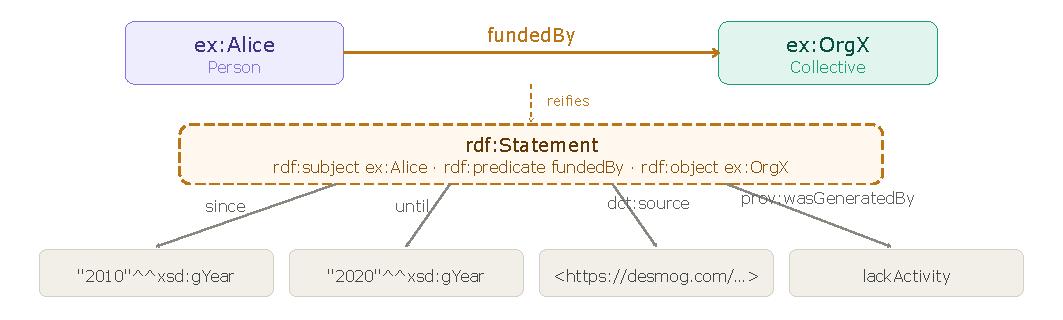
\includegraphics[width=\textwidth]{figures/lack-reification-diagram.pdf}
    \caption{RDF reification of a binary relation, decorated with temporal annotations (\texttt{since}, \texttt{until}), evidence source (\texttt{dct:source}), and provenance (\texttt{prov:wasGeneratedBy}).}
    \label{fig:reification}
\end{figure}

\paragraph{Availability.}
The LACK ontology is identified by the namespace URI \url{https://purl.net/climatesense/lack/ns#} and is available for download in Turtle and OWL Manchester Syntax formats.
It is published under a Creative Commons Attribution 4.0 International (CC BY 4.0) licence.
